\documentclass[a4paper]{article}

  \usepackage{fullpage} % Package to use full page
  \usepackage{parskip} % Package to tweak paragraph skipping
  \usepackage{tikz} % Package for drawing
  \usepackage{amsmath}
  \usepackage{amsfonts}
  \usepackage{amssymb}
  \usepackage{hyperref}
  \usepackage[utf8]{inputenc}
  \usepackage[english]{babel}
  \usepackage{multicol}
  \usepackage{mathtools}
  \usepackage{pgfplots}

  \usetikzlibrary{fit,shapes}

  \newcommand\tab[1][0.5cm]{\hspace*{#1}}
  \DeclarePairedDelimiter\ceil{\lceil}{\rceil}
  \DeclarePairedDelimiter\floor{\lfloor}{\rfloor}
  \pgfplotsset{compat=newest}
  
  \title{Discrete Mathematics: HW5}
  \author{Adrian Darian}
  \date{2018/10/19}
  
  \begin{document}
  
  \maketitle
  
  \section*{2.3 Functions}
  \begin{itemize}
    \item[8] Find these values. \\
      e. $\ceil{2.99} = 3$ \\
      f. $\floor{-2.99} = -2$ \\
      g. $\floor{\frac{1}{2} + \ceil{\frac{1}{2}}} = \floor{\frac{1}{2} + 1} = \floor{1.5} = 1$ \\
      h. $\floor{\frac{1}{2} * \floor{\frac{5}{2}}} = \ceil{0 + 1 + 0.5} = \ceil{1.5} = 2$
    \item[10] Determine whether each of these functions from $\{a, b, c, d\}$ to itself is one-to-one. \\
      a. $f(a) = b, f(b) = a, f(c)= c, f(d) = d$ \\
      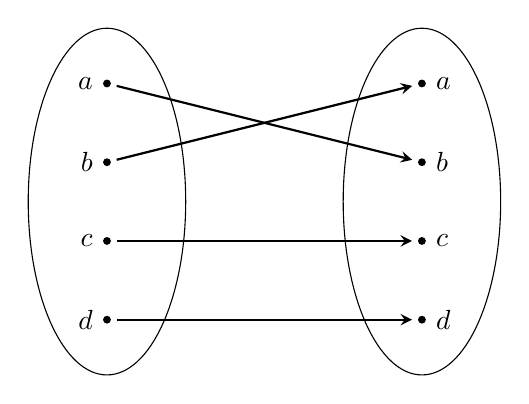
\begin{tikzpicture}[
        >=stealth,
        bullet/.style={
          fill=black,
          circle,
          minimum width=1pt,
          inner sep=1pt
        },
        projection/.style={
          ->,
          thick,
          shorten <=2pt,
          shorten >=2pt
        },
        every fit/.style={
          ellipse,
          draw,
          inner sep=0pt
        }
      ]
        \foreach \y/\l in {1/d,2/c/,3/b,4/a}
          \node[bullet,label=left:$\l$] (a\y) at (0,\y) {};
    
        \foreach \y/\l in {1/d,2/c,3/b,4/a}
          \node[bullet,label=right:$\l$] (b\y) at (4,\y) {};
    
        \node[draw,fit=(a1) (a2) (a3) (a4),minimum width=2cm] {} ;
        \node[draw,fit=(b1) (b2) (b3) (b4),minimum width=2cm] {} ;
    
        \draw[projection] (a4) -- (b3);
        \draw[projection] (a3) -- (b4);
        \draw[projection] (a2) -- (b2);
        \draw[projection] (a1) -- (b1);
      \end{tikzpicture} \\
      \tab function $f$ is one-to-one \\
      b. $f(a) = b, f(b) = b, f(c) = d, f(d) = c$ \\
      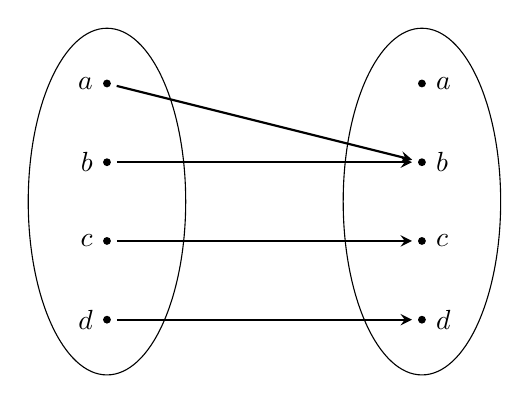
\begin{tikzpicture}[
        >=stealth,
        bullet/.style={
          fill=black,
          circle,
          minimum width=1pt,
          inner sep=1pt
        },
        projection/.style={
          ->,
          thick,
          shorten <=2pt,
          shorten >=2pt
        },
        every fit/.style={
          ellipse,
          draw,
          inner sep=0pt
        }
      ]
        \foreach \y/\l in {1/d,2/c/,3/b,4/a}
          \node[bullet,label=left:$\l$] (a\y) at (0,\y) {};
    
        \foreach \y/\l in {1/d,2/c,3/b,4/a}
          \node[bullet,label=right:$\l$] (b\y) at (4,\y) {};
    
        \node[draw,fit=(a1) (a2) (a3) (a4),minimum width=2cm] {} ;
        \node[draw,fit=(b1) (b2) (b3) (b4),minimum width=2cm] {} ;
    
        \draw[projection] (a4) -- (b3);
        \draw[projection] (a3) -- (b3);
        \draw[projection] (a2) -- (b2);
        \draw[projection] (a1) -- (b1);
      \end{tikzpicture} \\
      \tab function $f$ is not one-to-one 
    \item[12] Determine whether each of these functions from $Z$ to $Z$ is one-to-one. \\
      c. $f(n) = n^3$ \\
      \tab $f(n) = f(m)$ for $n, m \in Z$ \\
      \tab $\Rightarrow n^3 = m^3$ in $Z$ \\
      \tab $\Rightarrow n = m$ in $Z$ \\
      \tab $\therefore f$ is a one-to-one function \\
      d. $f(n) = \ceil{\frac{n}{2}}$ \\
      \tab $f(1) = \ceil{\frac{1}{2}} = 1$ and $f(2) = \ceil{\frac{2}{2}} = 1$ \\
      \tab $\therefore f$ is not a one-to-one function 
    \item[16] Consider these functions from the set of students in a discrete mathematics class. Under what conditions is the function one-to-one if it assigns to a student his or her \\ 
      a. mobile phone number. \\
      \tab any two students may not have the same mobile number \\
      b. student identification number. \\
      \tab each student's identification is unique and only has one identification number \\
      c. final grade in the class. \\
      \tab if there are less students than grades and each student has a different grade then the function is one-to-one \\
      d.  home town. \\
      \tab if more than one student has the same home town then it is not one-to-one
    \item[22] Determine whether each of these functions is a bijection from $R$ to $R$. \\
      c. $f(x) = \frac{(x + 1)}{(x + 2)}$ \\
      \tab the relation $f(x) = \frac{(x + 1)}{(x + 2)}$ from $R$ to $R$ fails as a function \\
      \tab $\therefore$ is not a bijection \\
      d. $f(x) = x^5 + 1$ \\
      \tab $f(x) = f(y)$ in $R$ \\
      \tab $\Rightarrow x^5 + 1 = y^5 + 1$ \\
      \tab $\Rightarrow x^5 = y^5$ \\
      \tab $\Rightarrow x = y \therefore it is one-to-one$ \\
      \tab $y = f(x) = x^5 + 1$ \\
      \tab $x = \sqrt[5]{y - 1}$ \\
      \tab $f(x = \sqrt[5]{y - 1}) = y \therefore$ it is a bijection
    \item[24] Let $f: R \rightarrow R$ and let $f(x) > 0$ for all $x \in R$. Show that $f(x)$ is strictly increasing if and only if the function $g(x) = \frac{1}{f(x)}$ is strictly decreasing. \\
    \tab $g(x) = \frac{1}{f(x)}$ \\ 
    \tab $x, y \in R$ \\
    \tab $x < y \Rightarrow \frac{1}{f(x)} > \frac{1}{f(x)}$ \\
    \tab $x, y \in R$ if $x < y$ then $f(x) < f(y)$ \\
    \tab $f(x)$ is strictly increasing if and only if $g(x) = \frac{1}{f(x)}$ is strictly decreasing.
    \item[36] Find $f \circ g$ and $g \circ f$, where $f(x) = x^2 + 1$ and $g(x) = x + 2$, are functions from $R$ to $R$. \\
    \tab $f(x) = x^2 + 1$ \\
    \tab $g(x) = x + 2$ \\
    \tab $(f \circ g)(x) = f(g(x)) = f(x + 2) = (x + 2)^2 + 1 = x^2 + 4x + 5$ \\
    \tab $(g \circ f)(x) = g(f(x)) = f(x + 2) = (x + 2)^2 + 1 = x^2 + 4x + 5$ 
    \item[46] Show that $\floor{x + \frac{1}{2}}$ is the closest integer to the number $x$, except when $x$ is midway between two integers, when it is the larger of these two integers. \\
    \tab $\floor{x} = n$ here$ x \leq x \leq n + 1$ \\
    \tab $\floor{x + \frac{1}{2}} = \floor{n + \epsilon + \frac{1}{2}}$ \\
    \tab $\Rightarrow \floor{n + \epsilon + \frac{1}{2}} = n$ \\
    \tab $\floor{x + \frac{1}{2}} = \floor{n + \frac{1}{2} + \frac{1}{2} + \epsilon_1}$ where $0 < \epsilon_1 < \frac{1}{2}$ \\
    \tab Hence $\floor{x + \frac{1}{2}} = \floor{n + 1}$
    \item[50] Show that if $x$ is a real number, then $x - 1 < \floor{x} \leq x \leq \ceil{x} < x + 1$. \\
    \tab $\ceil{x} = n$ if and only if $n - 1 < x \leq n$ \\
    \tab $\ceil{x + m} = n + m = \ceil{x} + m$
    \item[52] Show that is $x$ is a real number and $n$ is an integer, then \\
      a. $x \leq n$ if and only if $\ceil{x} \leq n$. \\
      \tab $x \leq \ceil{x}$ \\
      \tab $n < x$ and $x \leq \ceil{x}$ \\
      \tab if $x \leq n$ then $\ceil{x} \leq n$ \\
      \tab if $\ceil{x} \leq n$ then $x \leq n$ \\
      \tab $x \leq n$ if and only if $\ceil{x} \leq n$ \\
      b. $n \leq x$ if and only if $n \leq \floor{x}$. \\
      \tab if $n \leq x$ then $n \leq \floor{x}$ \\
      \tab $n \leq \floor{x}$ then $n \leq x$ \\
      \tab $n \leq x$ if and only if $n \leq \floor{x}$
    \item[66] Draw the graph of the function $f(x) = \ceil{x} + \floor{\frac{x}{2}}$ from $R$ to $R$. \\
    \begin{tikzpicture}
      \begin{axis}[
          axis lines=middle,
          xmin=-3,
          xmax=3,
          ymin=-7,
          ymax=10,
          enlarge y limits={abs=.6pt}, % very thick: 1.2pt
      ]
      \addplot [
          jump mark mid,
          domain=-3 - 1/6:3 + 1/6,
          samples=20,
          very thick, red
      ] {ceil(x) + floor(1/2)};
      \end{axis}
      \end{tikzpicture}
  \end{itemize}

  
  \section*{2.4 Sequences and Summations}
  \begin{itemize}
    \item[10] Find the first six terms of the sequence defined by each of these recurrence relations and initial conditions. \\
      b. $a_n = a_{n - 1} - a_{n - 2}, a_0 = 2, a_1 = -1$ \\
      \tab $2, -1, -3, -2, 1, 3$ \\
      c. $a_n = 3a^{2}_{n - 1}, a_0 = 1$ \\
      \tab $1, 3, 27, 2187, 14348907, 617673396283947$ \\
      d. $a_n = na_{n - 1} + a^2_{n - 2}, a_0 = -1, a_1 = 0$ \\
      \tab $-1, 0, 1, 3, 13, 74$
    \item[12] Show that the sequence $\{a_n\}$ is a solution of the recurrence relation $a_n = -3a_{n - 1} + 4a_{n - 2}$ if \\
      b. $a_n = 1$. \\
      \tab $n \geq 2$ \\
      \tab $-3(1) + 4(1) = 1 = a_n$ \\
      \tab $\therefore \{a_n\}$ where $a_n = 1$ is a solution of recurrence relation
      c. $a_n = (-4)^n$. \\
      \tab $-3(-4)^{n - 1} + 4(-4)^{n - 2} = (-4)^{n - 2}\{12 + 4\} = (-4)^{n - 2}(-4)^2 = a_n$
    \item[16] Find the solution to each of these recurrence relations with the given initial conditions. Use an iterative approach such as that used in Example 10. \\
      c. $a_n = a_{n - 1} - n, a_0 = 4$ \\
      \tab $a_n = a_{n - 1} - n$ \\
      \tab $1 + 2 + 3 + ... + n = \frac{n(n + 1)}{2}$ \\
      \tab $a_n = 4 - \frac{n(n + 1)}{2}$ \\
      d. $a_n = 2a_{n - 1} - 3, a_0 = -1$ \\
      \tab $a_n = -2^{n + 2} + 3$ \\
      e. $a_n = (n + 1)a_{n - 1}, a_0 = 3$ \\
      \tab $a_n = 2(n + 1)!$ \\
      f. $a_n = 2na_{n - 1}, a_0 = 3$ \\
      \tab $a_n = 3.2^{n}n!$
    \item[22] An employee joined a company in $2009$ with a starting salary of $\$50,000$. Every year this employee receives a raise of $\$1000$ plus $5\%$ of the salary of the previous year. \\
      a. Set up a recurrence relation for the salary of the employee $n$ years after $2009$. \\
      \tab $a_n = a_{n - 1} + 0.05a_{n - 1} + 1000$ \\
      b. What will the salary of this employee be in $2017$? \\
      \tab $a_8 = a_7 + 0.05a_7 + 1000$ \\
      \tab $a_8 = 83422$ \\
      c. Find an explicit formula for the salary of this employee $n$ years after $2009$. \\
      \tab $a_n = k_1(1.05)^n - 20000$ \\
      \tab $a_n = 70000(1.05)^n - 20000$ 
    \item[26] For each of these lists of integers, provide a simple formula or rule that generates the terms of an integer sequence that begins with the given list. Assuming that your formula or rule is correct, determine the next three terms of the sequence. \\
      d. $1, 2, 2, 2, 3, 3, 3, 3, 3, 5, 5, 5, 5, 5, 5, 5, ...$ \\
      \tab $1 1's, 3 2's, 5 3's$ and $7 5's$ \\
      \tab $(2n - 1)$ \\
      \tab The next three terms of the sequence are $7, 7$, and $7$, because the $7$ is repeated $9$ times. \\
      e. $0, 2, 8, 26, 80, 242, 728, 2186, 6560, 19682, ...$ \\
      \tab $a_1 = 0, a_{n + 1} = 3a_n + 2, n \in N$ \\
      \tab $59048, 177146, 531440$ \\
      f. $1, 3, 15, 105, 945, 10395, 135135, 2027025, 34459425, ...$ \\
      \tab $a_n = (2n - 1)a_{n - 1}, n\in N$ \\
      \tab $654729075, 13749310575, and 316234143225$ \\
      g. $1, 0, 0, 1, 1, 1, 0, 0, 0, 0, 1, 1, 1, 1, 1, ...$ \\
      \tab $0, 0, 0$
    \item[34] Computer each of these double sums. \\
      a. $\sum_{i = 1}^3 \sum_{j = 0}^2 (i - j)$ \\
      \tab $\sum_{i = 1}^3 (i - 1) + (i - 2) = \sum_{i = 1}^{3} (2i - 3) = (2 -3) + (4 - 3) + (6 - 3) = -1 + 1 + 3 = 3$ \\
      c. $\sum_{i = 1}^3 \sum_{j = 0}^2 j$ \\
      \tab $\sum_{i = 1}^{3} (\sum_{j = 0}^{2} j) = 3(0 + 1 + 2) = 9$
    \item[44] Express $n!$ using product notation. \\
    \tab $n! = 1 x 2 x 3 x ... x n = \prod_{i = 1}^{n} i$ 
  \end{itemize}

  
  \end{document}